\documentclass[sigconf]{acmart}

\usepackage{graphicx}
\usepackage{hyperref}
\usepackage{todonotes}

\usepackage{endfloat}
\renewcommand{\efloatseparator}{\mbox{}} % no new page between figures

\usepackage{booktabs} % For formal tables

\settopmatter{printacmref=false} % Removes citation information below abstract
\renewcommand\footnotetextcopyrightpermission[1]{} % removes footnote with conference information in first column
\pagestyle{plain} % removes running headers

\newcommand{\TODO}[1]{\todo[inline]{#1}}

\usepackage{hyperref}

\usepackage{endfloat}
\renewcommand{\efloatseparator}{\mbox{}} % no new page between figures

\usepackage{booktabs} % For formal tables

\settopmatter{printacmref=false} % Removes citation information below abstract
\renewcommand\footnotetextcopyrightpermission[1]{} % removes footnote with conference information in first column
\pagestyle{plain} % removes running headers


\begin{document}
\title{Big Data Analytics on Influencers in Social Networks}



\author{Bharat Mallala}
\affiliation{%
  \institution{Indiana University}
  \city{Bloomington, IN 47408} 
  \country{USA}}
\email{bmallala@iu.edu}

\author{Jyothi Pranavi Devineni}
\affiliation{%
  \institution{Indiana University}
  \city{Bloomington, IN 47408} 
  \country{USA}}
\email{jyodevin@iu.edu}


% The default list of authors is too long for headers}
%\renewcommand{\shortauthors}{B. Trovato et al.}


\begin{abstract}
Social Networking has become a part of people's lives with millions
of posts made every day. This huge volume of data paves the way to find interesting insights from data. Applying Big Data analytic methods on Twitter data helps in identifying the most influenced users.The Twitter data used for analysis is taken from Kaggle website. Performing feature selection tasks on this data has helped in identifying the important features that differentiate a user's influence over the other. By applying various Machine learning classification algorithms iteratively on these features obtained can be used to classify a user as more influential over the other. 

\end{abstract}

\keywords{I523, hid215, hid208, Machine Learning, Artificial Intelligence, Data Analysis, Multi layer Neural Network, Logistic regression, Random Forest Classifier, Support Vector Classifier(SVC), Stochastic Gradient Descent(SGD), K Nearest Neighbours(KNN), Naive Bayes.}
\maketitle
\section{Introduction}
Social Media is a powerful tool to express one's thoughts, ideas and experiences. With the exponential growth in active users across various social media platforms such as Facebook, Twitter, Instagram etc, a mammoth amount of data is being generated across these platforms. With such huge volume of data readily available, a lot of research is being carried on in the recent time in analyzing this data using various tools and extracting useful insights from it. With such large number of active users on these platforms, organizations are looking to capitalize on the opportunity to reach out to a large mass of population with absolutely low marketing costs.

Post made on Twitter are short and concise making it one the most used social media platform used by millions all around the world. Contrary to other social media platforms, Twitter has a limit on the number of words used by its users to make posts, making it the most professional way to interact with people. Most influenced people around the world such as politicians, sportsmen, businessmen, artists are active users of Twitter. With such large number of celebrities using Twitter to express themselves, it is interesting to find how influential they are when compared to their counterparts.

One can argue that a user's influence on Twitter is directly proportional to the number of followers he/she has. This is debatable as a set of people argue that with the number of followers a celebrity has, a post made by he/she influences a large population. While others argue that many others factors come into to picture when quantifying how influenced is a person rather than raw follower count. This can be analyzed by collecting a large volume of Twitter data and identifying the key factors that contribute to the influence of a user. Many methods are in use for collecting data from Twitter with the most popular ones being Twitter API and GOT3 or using readily available data online. Identifying influenced users across Twitter can be helpful in multiple domains. For example, this analysis can be used to formulate marketing strategies by organizations so that they can approach the more influenced people to make a post on their products for them to reach out to a large population. Also identifying most influenced persons during election campaigns can be used to predict the winning presidential candidate. Candidates can even deploy strategies to make themselves more influential on Twitter which indeed helps in their campaigning.

That data for the analysis is obtained from Kaggle data science competition. The train datasets has 5500 rows and 13 columns. The approach here is to classify each of users which has attributes from both the A user and the B user into tho classes making it a Binary classification problem. The data is split into train and test datasets using 5 fold cross-validation. This is because we do not have test data and to test the model performance we need test data to work with.Many approaches for binary classification such as Multilayer Neural Network, Logistic regression, Random Forest Classifier, Support Vector Classifier(SVC), Stochastic Gradient Descent(SGD), K Nearest Neighbours(KNN), Naive Bayes have been used to classify every row in the data into either of the two classes. The models are fitted on the train part of the split dataset and tested on the testing data set for obtaining the model accuracy.

Prior to fitting the models, it is important to obtain the features that are most useful for classification. Using all the features in the dataset is not a good approach as the model tends to memorizes the data points which eventually leads to overfitting. Random forest feature importance is used to rank the features in the dataset based on their importance towards the classification task. While there are many approaches towards feature reduction, Random forest is most followed approach giving the best possible results for the data in many situations. Then a subset of these features of the variable importance is taken for model fitting and discarding the remaining features. The random forest approach is run multiple amounts of times before feature selection since there is randomness involved in the approach and it is optimal to normalize the results from various iterations.

The above-stated models are then fitted on this subset of features in an iterative fashion. Various parameters of these models must be taken into consideration when fitting the models. The parameters should then be tweaked according to the data set and obtain the best parameter set for every model. Once the models are fitted it is important to evaluate the performance of these models and compare them against one another to obtain the best model that fits the data. the performance is tested on the test data obtained from the split using metrics such as accuracy score, precision score, recall score, F1 score and confusion matrix. These are various metrics that describe various properties of the performance of the model. 
\section{Literature Review}

Previous research on determining the user influence in twitter by Krishna P. Gummadi suggests that the indegree, retweets, and mentions play a major role in determining a user’s influence on Twitter. Where, in-degree refers to how popular a user is, re-tweets is the number of re-tweets received by a post made by the user and mentions is the number of mentions he got from his post. Krishna P. Gummadi says that a user being more popular may not be equally influential in terms of re-tweets and mentions. In his paper, he only used these three attributes to determine the influence of a user on Twitter.\cite{M2010}

Whereas, the approach proposed currently uses more attributes than that and hence is expected perform better than Krishna P. Gummadi’s model.  It is always better to have more attributes or more data so that we can then perform feature selection to select the most important features. We can also calculate the correlations between different features to see how they influence each other. It is better to consider re-tweets or mentions received and sent and also the follower as well as the following count to determine the influence to model a better classifier.\cite{M2010}

Katz, E., and Lazarsfeld discuss a useful method to determine the most influential customer using social network so that the companies to market their product to so that they can market it to an exponential number of people. They say that “ Instead of viewing a market as a set of independent entities, we view it as a social network and model it as a Markov random field”.  Their method focuses on calculating a network for a given customer. The current method proposed is an extension to this, predicting who is the most influential user, instead of calculating the network value of each user.\cite{Katz1955}



\section{Data Description}
The data for classification and analysis is taken from Kaggle's competition on "Influencers In Twitter". The idea was to use bigger data set, but due to scalability issues, have only used a smaller data set. The data set has 5500 rows and 23 columns. Each row in the data corresponds to two users A and B. Each row is independent t of one another i.e. the A user and B user in each row is independent of each other. The first column 'Choice' in the data set represents the class label. This column has a value of 1 if B user is more influential that the A user and has a value of 0 if A user is more influential that the B user. The next 11 columns belong to attributes of the A user followed by 11 columns belonging to the attributes of B user.

The following are the 11 attributes of each user:
\begin{enumerate}
    \item Follower-count
    \item Following- count
    \item Listed-count
    \item Mentions-received
    \item Mentions-sent
    \item Retweets-received
    \item Retweets-sent
    \item Posts 
    \item Network feature-1
    \item Network feature-2
    \item Network feature-3 
\end{enumerate}
\textbf{Follower count, Following count:} These attributes in the data specifies the number of users following the A or B user and number of users followed by user A or B respectively. \\
\textbf{Listed count:} This attribute specifies the number of private lists the A or B user is a part of.\\
\textbf{Mentions Received and Retweets Received:} These attributes specify the number of mentions and the number of re-tweets A or B user received from other users.\\
\textbf{Re-tweet Sent:} specifies the number of re-tweets A or B user sent to other users.\\
\textbf{Post:} This attribute describes the number of tweets made till date by the users.\\
\textbf{Network feature attributes:} These are obtained as a result of PCA analysis and are included in the data. They correspond to some variance in the data from the network point of view.


\section{Feature Selection}

Due to the existence of a large number of features available in the data set, this feature should be reduced and only the most important features that help to model the data needs to be selected. If all the features are used to model the data the model performs exceptionally well on the training data set but fails to perform well on the testing data set. This is called 'Over-fitting'. This a general phenomenon that occurs across most Machine learning algorithms when using a large set of feature for classification because the model learns to memorize these features resulting in a good accuracy score for train data set, but when we encounter a new set of values for these features in the testing data the models fail to classify them correctly resulting in a poor accuracy score.

There are many approaches to feature selection. One approach is to have domain knowledge on the data i.e. having prior knowledge on the data set and by intuition selecting features from the data. For example, if we are predicting sales prices of a house based on the features of the house, having an in-depth knowledge on what feature make the house price go up or down can help is selecting the features of interest. This often requires a professional who experts in that domain to make the decision. But this approach often fails for two reasons, firstly it hard to find an expert opinion on every data set and secondly the intuition of the expert can be trusted as human are prone to make mistakes in estimation.

The ideal approach would be to use some algorithm that can predict the features of interest by iterating over the model multiple times. Random forest for feature selection is one such algorithm. As the word random suggests, the algorithm builds small decision trees using a different subset of features in each iteration and then combines the insights from all of these decision trees and ranks the features in the dataset based on their importance. Since the algorithm builds thousands of trees based on the random selection of features, the feature ranking, for the most part, is accurate. One the features with its ranking are obtained, one has to select a subset of these features and use them for model classification. Since the ideal number of features that best suits the model is still unknown, the approach is to iterate over the important feature and select the best possible subset. For the Twitter dataset, the random forest ranked the feature according to their importance and selecting 8 of the top most important feature given the best possible results.
The features are follower count, listed count, re-tweets received and Network features 1 for both A and B users. The figure 7 shows the features ranked according to their importance.


\section{Classification methods}
Since we have only two classes (either 0 or 1) in our class label, it becomes a binary classification problem. A lot models can be used for binary classification. The approach is to fit 8 of these models for the data set and evaluate the performance of each of these models by using the evaluation metrics.

\subsection{Logistic Regression}
Logistic regression is one of the Generalized Linear Models that describes the relationship between the response variable and the explanatory variables\cite{Agresti2007}. The response variable can either be binary or multinomial. If the response variable is binary, it is called binary logistic regression and if it is multinomial, it is called multinomial logistic regression. 
The  cumulative distribution function for logistic regression is given by:
\begin{equation}
    F(x) = P(X \leq x) = \frac{e^{\frac{(x-\mu)}{\tau}}}{1+e^{\frac{(x-\mu)}{\tau}}}
\end{equation}
Where $\mu$ is the mean of the given set of data points and $\tau$ is a scaling parameter.\\
Using the cumulative distribution function for logistic regression\cite{Agresti2007}, the logistic regression function is given by:
\begin{equation}
    log(\frac{\pi(x)}{1-\pi(x)}) = \alpha + \beta x
\end{equation}
where:
\begin{equation}
    \pi(x) = \frac{e^{\alpha+\beta x }}{1+e^{\alpha+\beta x }}
\end{equation}
$\pi$ is the probability of occurrence of an event. Where\\
\begin{equation}
    \alpha = -\mu/\tau
\end{equation}
\begin{equation}
    \beta = 1/\tau
\end{equation}

    

The relationship between $\pi(x)$ and x is mostly non-linear. The influence of x on $\pi(x)$ is more when it is near 0 or 1 rather than when it is in between. $\pi$ either increases or decreases with an increase in x\cite{Agresti2007}. The rate of increase or decrease depends on $\beta$. If $\beta$ $>$ 0, then $\pi(x)$ increases with an increase in x and if $\beta$ $<$ 0, then $\pi(x)$ decreases with an increase in x and remains constant when $\beta$ = 0.\\
The random component for the response variable in logistic regression has a binomial distribution. The link function is 'logit'. The logistic regression model is also sometimes referred to as logit model. If it is a multinomial logistic regression model, then the random component would be multinomially distributed\cite{Agresti2007}.
\subsection{Random Forest Classifier}
The Random forest algorithm apart from its use as feature selection method can also be used a Classifier. Random forest in one of the ensemble classification methods currently in use."Ensemble learning is a machine learning paradigm where multiple learners are trained to solve the same problem"\cite{Zhou2016}. Typical methods for example Decision tree algorithm build trees by iterating over the features in the train data set. But ensemble method uses a different approach, for example, Random forest build a number of small decision trees based on a subset of training features and combine the results from all these decision trees and obtain a better accuracy. It eventually builds a forest of decision trees, hence the name Random Forest.\cite{Breiman2010}

Each of the decision trees has a decision as two which class a new data point belongs to. Random forest algorithm classifies the data point by combining the decisions from all the decision trees. Hence it provides better performance while at the same time over-fitting on most occasions. The random forest classifier has two stages, the training phase, and the classification phase. \cite{Breiman2010}

In the training phase from the corpus of training features, a random subset of features is sampled with replacement. Three-fourths of the data is sampled leaving out the remaining data for formulating the classification error. It is called out of bag data (OOB). In the classification phase, proximities are calculated for every decision tree for each of the two classes. If two decision trees have the same proximities for each of the two classes the proximity is increased by one. Once all the proximities are determined it is then divided by the total number of decision trees to normalize it.\cite{Breiman2010}

While building the decision trees typically the Gini importance is used.Gini index splits the tree based on whether the Gini impurity criterion of the current node is less than the parent node.

\begin{equation}
    I_G(p) = 1-\sum_{i=1}^{J} (p_i)^2
\end{equation}\\

Where $I_G(p)$ is gini impurity of p\\
J is the number of classes (J=2 for binary classifiaction)
$p_i$ is the number of items classified into class i\\
Here there are a few design choices to be made\\
\textbf{Max iterations:} - Have to specify the maximum number of iterations the classifier has to run. It is hard to find an optimal number for every problem. Need's to be iterated across multiple values. 
\textbf{Max depth:}- Specifies the maximum depth to which he decision tress are built.\\
\textbf{N estimators:}- specifies the maximum number of trees built in each iteration.\\
\textbf{Max features}- specifies the number of features to be considered when splitting the decision tree.\\
\textbf{Criterion} - specifies using either gini impurity index or entropy. By default it uses gini impurity index.\cite{Breiman2010}


\subsection{Stochastic Gradient Descent}
Gradient descent is one of the machine learning algorithms which is used for updating the weights of a neural network to optimize the prediction error of machine learning algorithms\cite{Brownlee2017}. The weights are updated so that the classification or regression error of training samples is minimized over the iterations. Gradient descent is classified into three types based on the number of training samples used for updating the weights. They are:
\begin{enumerate}
    \item Batch Gradient Descent
    \item Stochastic Gradient Descent
    \item Mini-batch Gradient Descent
\end{enumerate}
In batch Gradient descent, the weights of the network are assigned randomly initially and the model is designed by updating the weights according to minimize the prediction error after all the training samples are classified\cite{Brownlee2017}.  \\
Stochastic Gradient Descent is another type of gradient descent in which the error is calculated for each training sample. The weights are updated for every training sample. Because of the kind of update the Stochastic Gradient Descent uses, it is called as online machine learning algorithm. There are both advantages and disadvantages of using this approach. One of the advantages is that the model is less prone to arrive at local minima as the update process is noisy\cite{Brownlee2017}. As the error is calculated frequently, the error in the prediction can corrected at that stage itself, instead of propagating it to next stages. Also, the frequent updating of weights may result in fast learning. On the other hand, one of the major disadvantages of this approach is that updating the weights for every training sample may be much time consuming and delay the convergence. Also the updates being noisy might cause the algorithm to arrive at a error minimum with high variance\cite{Brownlee2017}.\\
To combine the advantages of both Batch Gradient Descent and Stochastic Gradient Descent, Mini-batch Gradient Descent can be used\cite{Brownlee2017}. In this method, the training data is divided into a number of subsets and the error is calculated and weights are updated for each subset. 
\subsection{Support vector Classifier}
Support Vector Machines is an advancement over Neural Network. A neural network converges if the two classes are linearly separable. Every time we run a neural network on the train data and plot the points and the line on a 2-D plane, we get a different line that separates the two classes, this happens due to the randomness in the initial weights chosen for the perceptrons. Since we get a different classifier every time we run it, it is obvious that one classifier is better than the other. The neural network does not guarantee the best possible classification. This is where SVC shines with its improvements over neural networks. SVC can be used both for classification and regression tasks but are typically used for classification. There mainly three types of SVC,\\\cite{Williamson2}
\textbf{1.Linear SVC}\\
\textbf{2.Nu SVC}\\
\textbf{3.SVC}\\

Ideally, the goal of SVC is to place the decision boundary i.e. the line that separates the two classes as far away from the classes as possible. The distance between the decision boundary and the data points in each class is called margin. Most often some of the data points exist within the margin and are close to the boundary, these points are called as 'Support vectors'. The distance from the vector to the boundary is given by,\cite{Williamson2}
\begin{equation}
    r = \frac{g(x)}{||w||}
\end{equation} 
where,
\begin{equation}
    g(x) = w^Tx+b
\end{equation}
where r is the distance, g(x) is the decision boundary and $||w||$ is the absolute value of the weight vector and b is the bias.

Since the goal here is to find the optimal decision boundary, the corresponding w and b should be estimated. This can be achieved by using the Primal problem which is a constraint minimization problem. The formulation of this is,\cite{Williamson2}

\begin{equation}
    d_i(w^Tx_i +b) \geq 1\\
\end{equation}
\begin{equation}
      \Phi(w) = \frac{1}{2}ww^T
\end{equation}

The above minimization can be solved using the Lagrangian formulation,

\begin{equation}
    J(w,b,\alpha) = \frac{1}{2}ww^T - \sum^{N}_{i=1}\alpha_i[ d_i(w^Tx_i +b)-1]
\end{equation}

where $\alpha_i$ is called the Lagrangian multipliers. We obtain the optimal values of w and b by partially derivating the above equation and equating it to zero. We get,
\begin{equation}
    w = \sum_i \alpha_id_ix_i
\end{equation}
\begin{equation}
    Q(\alpha) = \sum_i \alpha_i - \frac{1}{2}\sum_i\sum_j \alpha_i\alpha_jd_id_jx_i^Tx_j
\end{equation}

here $\alpha_i$ > 0 only for support vectors and Q is quadratic.\\
Finally after getting $\alpha_i$, the optimal $w_0$ is,
\begin{equation}
    w_0 = \sum_{i=1}^{N_s} \alpha_0d_ix_i
\end{equation}

where $N_s$ is the number of support vectors. 
\begin{equation}
    b_0 = \frac{1}{d^(s)} - w_0^Tx^{(s)}
\end{equation}

Since now we have the optimal value for w and b, we get the optimal decision boundary. SVC generally gives a better accuracy over perceptron and it can be used efficiently for high dimensional planes.\cite{Williamson2}
\subsection{Multi layer Perceptron}

The neural network came into existence in the early 1960's but was not very popular approach since it had some limitations in solving complex problems. But with the introduction of backpropagation algorithms and its application on Multi-layer Neural networks. Each neural network comprises of individual neurons which are also called perceptions. These neurons are connected to one another with edges. A simple neural network has three layers, input layer, an output layer and the hidden layer. The inputs layers consist of data points these data points are connected to the neuron in the hidden layer by an edge which has weights and biases associated with them. The hidden layer is then connected to the output layer with edges which also has weights and biases.\cite{Williamson1}

Based on the type of the problem, the output layer either output a binary value(0 or 1) or any continuous value. The input data point is multiplied by the weight of the neuron and the bias of that neuron is added. All output from each neuron is added together and is fed to an activation function and produces an output. Once an iteration is completed the weights of the network are updated based on the output obtained from the first iteration using the perceptron learning algorithm. The learning stops when there is no significant improvement from one iteration to the other. The error is calculated after each iteration which quantifies the number of misclassified data points.
\cite{Williamson1}
\begin{equation}
   w(n+1) = w(n) + \eta[d(n)-y(n)]*x(n)
\end{equation}
where,\\
w(n+1)-new weight of the neuron\\
w(n)- old weight of the neuron\\
d(n)- desired output\\
y(n)- acutal output\\
x(n)- data point\\\\

This simple neural network can only be used yo solve a handful of problems. For example, it cannot solve the XOR problem. To deal with much more complicated problems we require the use of Multi-layer Neural networks with the back-propagation algorithm to update the weights in each iteration. The back-propagation algorithm uses gradient descent to update the weights by cost minimization. There are two steps in the back-propagation algorithm. One is the feedforward step where the network feeds forward and find the output. In the back-propagation step the algorithm back-propagates and update the weights in each layer by using gradient descent. This is done is a backward fashion starting from the output layer and then the hidden layers. There are two methods for updating the weights, batch update and the online update. While batch update method updates the weights after one iteration of all the data points, the online update method updates the wights after each data point is passed through the network.
\cite{Williamson1}
Here there are lot of design choice to made\\
1.Initializing weights - weights are usually initialized random normal manner. \\
2.Choosing the number of hidden layers- This parameter cannot be determined in advance. One has to iterate through multiple values of the hidden layer unless the best accuracy is obtained.\\
3.Update method- The weights can be updated typically using the batch update on the online update. In most application typically the online method is used as it is much more efficient.\\
4.Choosing the Activation function- This is a difficult task, most commonly non-linear activation functions are used. Example Re-Lu activation function.
\cite{Williamson1}
The figure shows the typical architecture of a Multi-layer Neural network. 

\subsection{K Nearest Neighbours}

K Nearest Neighbours is one of the simplest machine learning models that can be easily implemented and it surprisingly works well for most classification problems. K Nearest Neighbours can be used for both classification and regression problems giving it the flexibility to solve most problems.

The algorithm assumes all the data points are scattered on a 2-dimensional plane and it tries to find clusters of these data points. The algorithm mainly has two phases, the training phase, and the classification phase. The training phase of KNN is fairly simple as it just stores the values of each of the variables and also the class label. The classification phase is the most important one as all the calculation are made in this phase. Since cross-validation is being used to split the data set into train and test, in the training phase the algorithm stores the values of each of the 8 attributes used for model fitting and also the values of the class label for each fold of the cross-validation.

In the classification phase for each data point in the test data set, the algorithm iterates over all the data point in the train data set and finds the k nearest neighbors to the current data point by calculating the distance between them. A variety of distance metrics can be used to find the nearest neighbors. The most commonly used ones are Manhattan Distance and Euclidean Distance. But based on the type of data other distance metrics can be used to obtain better performance. Once the k nearest neighbors are obtained the algorithm looks for the class labels for these neighbors and assigns the most occurring label among these neighbors to the current data point. This happens for every data point in the test data set and every fold in the cross-validation. The algorithm then assigns the most occurring class labels across all folds.

The value of k is unknown for a given problem and one has to iterate over multiple values of k to find the best accurate model.The most common approach to find k is to iterate over multiple values of k starting from 1 and stopping when the difference in performance from the previous value of k is below a certain threshold. This threshold can be set based on the type and volume of data. Ideally, the threshold should not be too large or too small. Some advantages of this model involve low training cost and it often works well with enough training data and a good distance metric. It also has few drawbacks which involve choosing the apt distance metric can be cumbersome without prior knowledge, it is easily prone to over-fitting and usually takes a lot of time and memory for the classification phase.

\subsection{Naive Bayes}
Naïve Bayes is one of the machine learning algorithms. It is known for its simplicity. It is a classification approach based on the Baye’s law. In this approach, prior knowledge is very essential. The basic idea is to compute the prior of each class and the likelihoods. Then, the posterior probabilities are calculated using Baye’s law for each class and the data point is assigned to the class with highest posterior probability. The prior represents the probability of occurrence of a class among all the given classes. The likelihoods or likelihood probabilities are a measure of how likely is a given data point prone to belong to a given class. Posterior probability is the probability of a class is one of the given classes, given a set of data points.\cite{Crandall} \\
There are two phases in the Naïve Baye’s classification as that of any other machine learning algorithm, training, and testing.  In the training phase, the prior probabilities of the classes are calculated by computing the number of times the class has occurred in the given data among all the classes. If there are n classes $C_1$, $C_2$,….$C_n$ and m data points $X_1$, $X_2$,….$X_m$, then the prior of a class is represented by P($C_i$) for I ranging from 1 to n. After computing the priors, the likelihood of each data point belonging to each one of the classes are calculated. The likelihood ratio is given by:\cite{Crandall}
\begin{equation}
    P(X_j/C_i) = \frac{P(X_j, C_i)}{P(C_i)}
\end{equation}
where i = 1 to n, j = 1 to m\\
Where, P($X_j$, $C_i$) is the probability of occurrence of the data point $X_j$ in class $C_i$. $X_j$ represents the $j^{th}$ data point in a given set of data points and $C_i$ represents the $i^{th}$ class.\cite{Crandall}\\
In the testing phase, the posteriors probabilities are using the Baye’s law:
\begin{equation}
    P(C_i/X_j) = \frac{P(X_j/ C_i) P(C_i)}{P(X_j) }	
\end{equation}
Where, P($X_j$) represents the total probability of $X_j$, given by:
\begin{equation}
    P(X_j) = \sum_{i=1}^{n}P(X_j/ C_i)P(C_i)
\end{equation}
Naive Bayes model makes the assumption that the data points are conditionally independent of each other given the class or label. Hence, the likelihood probability of a set of data points belonging to a class becomes:\cite{Crandall}
\begin{equation}
    P(X_1,X_2,. . . X_n/Ci) = \prod_{j=1}^{n} P(X_j/C_i)
\end{equation}
Then the posterior probability of a set of data points can be written as:
\begin{equation}
    P(C_i/X_1,X_2,. . . X_n) = \frac{\prod_{j=1}^{n} P(X_j/C_i) P(C_i)}{P(X_1,X_2,. . . X_n) }	
\end{equation}
For a given set of data points, P($X_1$,$X_2$,. . . $X_n$) remains constant and hence, equation(6) can be written as:
\begin{equation}
    P(C_i/X_1,X_2,. . . X_n) \propto \prod_{j=1}^{n} P(X_j/C_i) P(C_i)
\end{equation}
Naive Bayes derives its name from making the naive assumption that the data points are conditionally independent of each other.There are three types of Naive Bayes classifiers:\cite{Crandall}
\begin{enumerate}
    \item Gaussian Naive Bayes
    \item Multinomial Naive Bayes
    \item Bernoulli Naive Bayes
\end{enumerate}
Gaussian Naive Bayes can be used for the classification when the given set of data points have Gaussian distribution.\cite{scikit-learn}\\
Multinomial Naive Bayes can be used when for the data if it is multinomially distributed\cite{scikit-learn}.
Bernoulli Naive Bayes can be used when all the attributes or features in a given data are binary\cite{scikit-learn}.
\subsection{AdaBoost}
Ensemble learning is one of the machine learning methods which is based on decision trees. The basic idea is to create an ensemble of hypotheses and combine their predictions instead of predicting using a single hypothesis\cite{Brownlee2016}. Boosting is one of the ensemble methods which attempts at learning a strong classifier from a set of weak classifiers. At first, an initial model is created and then the next model attempts to correctly classify the training samples which have been misclassified by the previous model. This process continues until a predefined number of models have been generated or there is nothing much to be done with the training data. \\
AdaBoost is one of the Boosting algorithms which is used for binary classification. It can only be used when the response variable is binary. AdaBoost can be used with any machine learning algorithms to improve the performance. It is most commonly used with decision trees. The decision trees used in AdaBoost are only of depth one, i.e., they only have one decision to make. Hence, the decision trees in AdaBoost are called decision stumps\cite{Brownlee2016}. \\
There are two phases in the AdaBoost as well, like any other machine learning algorithms. In the training phase, all the given training samples are assigned with uniform weights. If there are n training samples, then each sample is given a weight of 1/n. Hence, the initial weights of the training samples can be written as\cite{Brownlee2016}:
\begin{equation}
    w(x_i) = \frac{1}{n}
\end{equation}
Where $x_i$ is the $i^{th}$ training sample and  w($x_i$) is the initial weight of $i^{th}$ training sample. Using these weighted samples, a weak binary classifier is modeled which can only make one decision and output either -1 or 1, where 1 represents the first class and -1 represents the second class. Then, the misclassification rate is calculated for the trained model as follows\cite{Brownlee2016}:
\begin{equation}
    error = \frac{(c-n)}{n}
\end{equation}
Where c is the number of correctly classifies samples and n is the total number of training samples. Now, weighted aggregate of the misclassification rate is calculated to further use it to modify the weights of the training samples. It is modified as\cite{Brownlee2016}:
\begin{equation}
    error = \frac{\sum_{i=1}^{n}w(x_i)e(i)}{\sum_{i=1}^{n}w(x_i)}
\end{equation}
Where e(i) is the prediction error of the $i^{th}$ training sample which is either 1 or 0. It is 0 if the sample is classified correctly and 1 if it is misclassified. \\
Then, stage value is calculated from the aggregated error as follows\cite{Brownlee2016}:
\begin{equation}
    stage = ln(\frac{1-error}{error})
\end{equation}
The stage value is used to assign greater importance to classifiers which are more accurate. The weights of the training samples are updated using the stage value so that samples which are correctly classified have less weight and the incorrectly classified samples have more weight. The weights are updated using the below equation\cite{Brownlee2016}:
\begin{equation}
    w(i) = w(i)*e^{stage*e(i)}
\end{equation}
We can observe from the above equation that if a sample i is correctly classified, then prediction error of that sample e(i) will be 0 and hence the weight of the sample remains as it is. Whereas, if the sample is misclassified, then e(i) would be 1 and the weight of the sample increases by a factor $e^{stag}$. This process is continued by updating the weights and modeling weak classifiers until a predefined number of weak classifiers have been modeled or when there is nothing more to be gained from the training data.\cite{Brownlee2016}\\
In the testing or prediction phase, when a test sample is to be classified into one of the two available classes, it is classified using all the weak classifiers designed in the training phase and the predicted values are given weights according to the stage value of the corresponding classifiers\cite{Brownlee2016}. The final predicted value is taken to be 1 if the weighted sum of these predicted values is positive and -1  if the sum is negative.

\section{Exploratory Data Analysis}
\subsection{Missing values}
Since the data is sparse, null values can exist in the data. These null values if not treated can be catastrophic to the model accuracy. The null or missing values can be treated either by removing the rows which have these values or replacing them with apt data. For example, if a data frame has 10 null values in a column, the approach would be to replace the values with either the mean, median or mode of that column.  The data here does not consist of any null or missing values in any of the rows.

\subsection{Outliers}
If a data point diverges very much from the rest of the data points it is called an outlier. These outliers if not addressed will eventually lead to overfitting of the model i.e. the model fits each and every point in the train data and gets a good accuracy, but when tested on unseen data it will result in a poor accuracy score. To overcome overfitting the outliers need to be addressed. The outliers in the data can be identified by either plotting a box plot or scatter plot of each of the variables in the train data and check for the distribution of data points.

Just like missing values the outlier can either be deleted from the data or can be modified to better suit the model. The ideal approach would be to use binning of the columns which have outliers. In binning data, we bin the data into small categories based on a range. The Twitter data here consists of a few outliers in almost all the attributes. Binning the data improved the accuracy score of all the models. The figure 6 shows the scatter plot of A follower count variable with outliers. From the scatter plot it is evident that for all the attributes the data point is concentrated in the lower range. Hence after binning each attribute into two the first two lower categories, null values are generated in the higher categories. Hence the rows with Null values have been dropped thereby removing the outliers. The data is reduced to 5209 rows after the removal of outliers. 

\subsection{Correlation among attributes}

Since the data consists of 22 columns apart from the class label, correlations among these attributes might be. Correlation is the measure of association between two attributes. It indicates how closely two attributes are related to each other. The range of correlation is between -1 and 1. A positive correlation indicates the two variables are directly proportional and a negative correlation indicated that they are indirectly proportional. If the value is zero then there is no association between the attributes.\\
The figure shows a heat map displaying the correlation among the variables. The color of the heat map indicates the level of correlation among attributes. As the color tends to get closer to yellow, it shows a positive correlation and shows a negative correlation if color tends to get bluer. For example, there is a strong correlation between network feature 1 and mentions received. This correlation also helps in feature selection as we can ignore one of the two features if they are closely related. The variables which are closely related to the class label are found to be follower count and listed count of both A and B. This is not very surprising as a person with high follower count or listed count on Twitter is expected to be more influential than others. These insights proved to be useful in the further analysis when performing feature reduction.
\section{Experiment and Results}
To avoid overfitting, the training data has been further split into train and test using cross-validation. 80 percent of the data has been used for training the classifier and the remaining 20 percent is used to evaluate the performance of the classifier. \\
Feature selection has been performed on the train data using Random Forest Classifier to obtain the most important attributes. A bar plot has been plotted to know the top most important variables which are shown in the figure. The top four important attributes are identified to be follower-count, listed-count, mentions-received and network feature-1 of both A and B. Further analysis or classification has been performed on these eight attributes.
\subsection{Evaluation Metrics}
One the model is fitted, there is a need to evaluate the performance of the model. Various evaluation metric can be used to measure how well the model performs. Accuracy score, precision score, F1 score, Confusion matrix and recall score are the most commonly used metrics to evaluate the performance of classifiers.They indicate various measure of evaluation\\
\textbf{1. Accuracy score:} Ratio of number of correctly classified data points to total number of data points.\\
\textbf{2. Precision score:}  Ratio of True positives to sum of True positives ,False positives for each class.\\
\textbf{3. F1 score:} Twice the ratio of product of precision and recall to the sum of precision and recall for each class.\\
\textbf{4. Recall score:} Ratio of True positives to sum of True positives ,False negatives for each class\\
\textbf{5. Confusion matrix:} To know how well the classifier performs in each class in the data. It gives the number of True positive, False positives, True negatives, and False negatives. The rows in the matrix correspond to actual class label and the columns to the predicted class label.\\\\
If a classifier has very high precision then it may miss many true instances of a label, similarly, if it has very high recall score it is prone to misclassify many data points. Hence a good classifier should have a trade-off between precision score and recall score.\\
For the Influence analysis, the Ada boost Classifier has the best performance with an accuracy score of 0.78 and an F1 score of 0.78. The MLP classifier performed the worst with an accuracy score of 0.68 and an F1 score of 0.67. This is because the classifier performed extremely well in one class and very poorly in the other class. This is evident from a high precision score in class 1 and a low recall score, and vice-versa for class 0. Whereas for the AdaBoost classifier both class 1 and 0 have decent precision and recall scores, hence finding a good trade-off between them. The figure 5 shows the evaluation performance of each classifier with all the evaluation metrics.  
\section{Future work}
Predicting the Influence of users based on various attributes paves the way for much more research in the area. Instead just classifying two users based on their influence it can be extended to a larger audience, which can be quite interesting. But it becomes a regression problem rather than a classification problem. This analysis can also be extended to address how an individual is influential i.e. in a good or a bad way. This can be achieved with the help of sentiment analysis performed on the users. But this would require the actual tweets that the users make.

\section{Conclusion}
Twitter being one of the most popular social media platforms, serves as a source for various thoughts expressed by people across different domains. These tweets or tweet data if analyzed in an efficient way can answer many questions. One of such questions is which user on Twitter is more influential. Given the tweets made by the user and other statistics like a number of retweets received, follower count, etc the user with more influence can be predicted using various machine learning classification techniques. AdaBoost is found to be the most efficient classification technique for this research question with an accuracy score of 0.78 and the least appropriate method was found to be the Multi-Layer Perceptron classification.  


\begin{acks}
We would like to thank Dr. Gregor von Laszewski and the AI's for all the help they have provided for this project..
\end{acks}

newpage
\appendix 
\section{Work Breakdown} 
\begin{description} 
\item[Dataset identification:]Bharat Mallala
\item[Exploratory data analysis:] Bharat Mallala and Jyothi Pranavi Devineni
\item[Feature Selection:] Jyothi Pranavi Devineni
\item[Random Forest, SVM, K nearest neighbours, MLP :] Bharat Mallala
\item[Naive bayes, SGD, Logistic regression, Adaboost:] Jyothi Pranavi Devineni
\item[Project Report:] Bharat Mallala and Jyothi Pranavi Devineni
\end{description} 

\bibliographystyle{ACM-Reference-Format}
\bibliography{report} 

\clearpage
\begin{figure}[htp]
    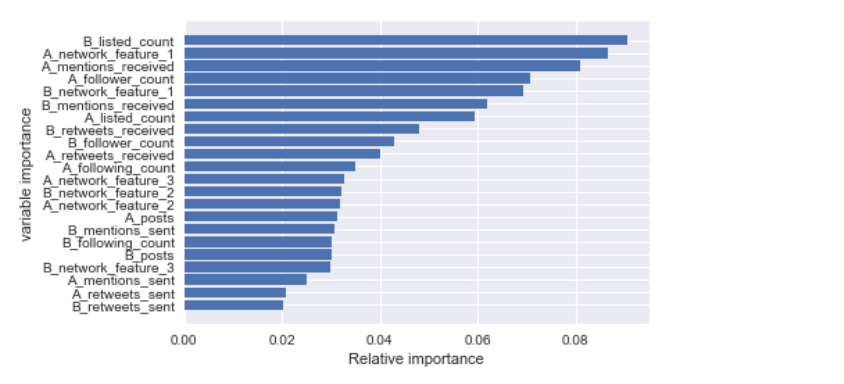
\includegraphics[width=0.8\textwidth]{Variable.PNG}
    \caption{Variable importance plot}
    \label{fig:figure1}
\end{figure}

\begin{figure}[htp]
    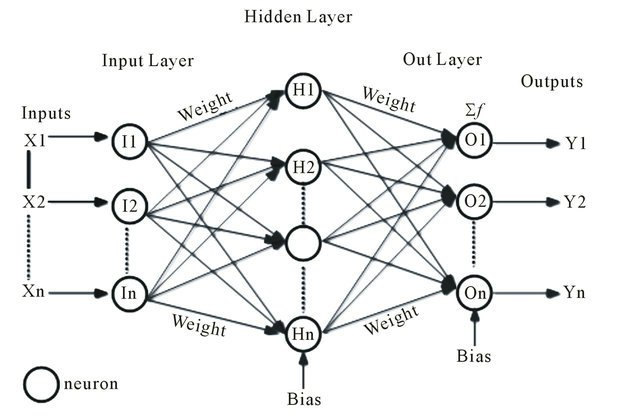
\includegraphics[width=1\textwidth]{neuralnet.jpg}
    \caption{Neural Network Architecture \cite{google1}}
    \label{fig:figure2}
\end{figure}

\begin{figure}[htp]
    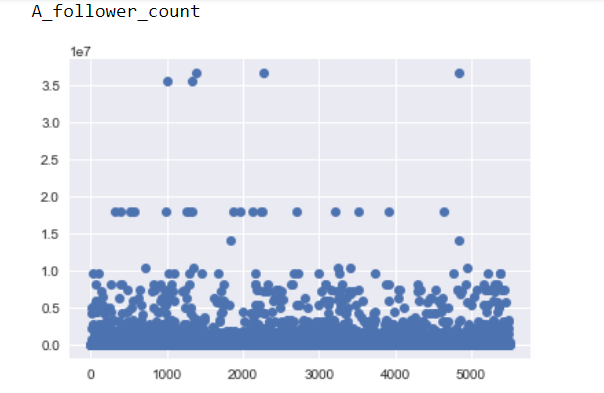
\includegraphics[width=0.8\textwidth]{Scatterplot.png}
    \caption{Scatter plot for follower count of A }
    \label{fig:figure 3}
\end{figure}

\begin{figure}[htp]
    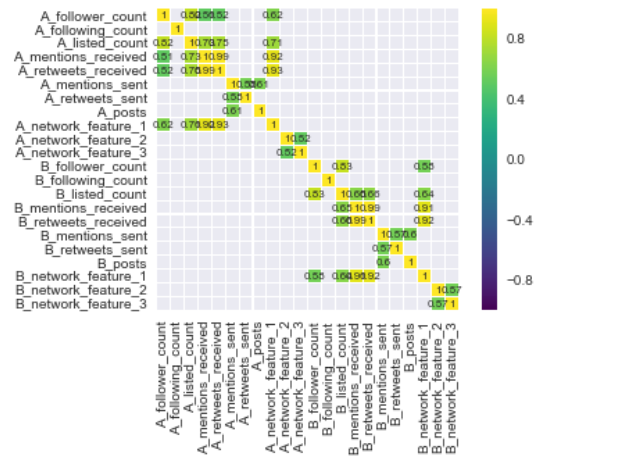
\includegraphics[width=0.8\textwidth]{heatmap.PNG}
    \caption{Heat Map showing correlation among variables}
    \label{fig:figure4}
\end{figure}



\begin{figure}[htp]
    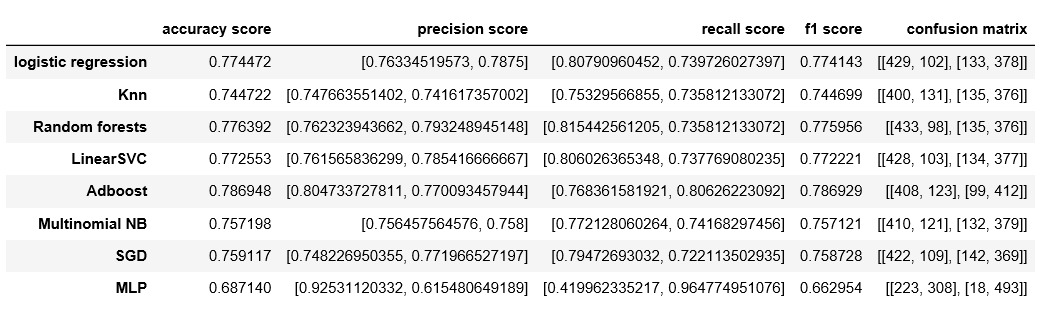
\includegraphics[width=0.8\textwidth]{results.jpeg}
    \caption{Model Performance}
    \label{fig:figure 5}
\end{figure}



\end{document}
